\chapter{Primera evaluación}

\section{Conjuntos numéricos}

\subsection{Conjuntos numéricos: Naturales, enteros, racionales y reales}

\subsection{Propiedades algebraicas}

\subsection{Propiedades de las fracciones}


\subsection{Exponentes enteros y fracciones algebraicas}


	[Simplificación de exponentes enteros]: Simplifique la siguiente expresión algebraica:
	\begin{align}
		\left(\frac{q^{-2} r s^{-2}}{r^{-5} s q^{-8}}\right)^{-1}  
			&= \frac{(q^{-2} r s^{-2})^{-1}}{(r^{-5} s q^{-8})^{-1}} \\
			&= \frac{q^{2} r^{-1} s^{2}}{r^{5} s^{-1} q^{8}} \\
			&= \frac{q^{2} r^{-1} s^{2}}{r^{5} s^{-1} q^{8}} \\
			&= \frac{r^{-1}}{r^5} \cdot \frac{q^2}{q^8} \cdot \frac{s^2}{s^{-1}} \\
			&= (r^{-1} \cdot r^{-5}) \cdot (q^2 \cdot q^{-8}) \cdot (s^2 \cdot s^1) \\
			&= r^{-6} \cdot q^6 \cdot s^{3} \\
			&= \frac{s^3}{q^6 r^6} \\
	\end{align}
	\qed


\subsection{Exponentes fraccionarios, propiedades de la radicación}


	[Racionalización de \(\frac{1}{\sqrt 2 }\)]: 
	\begin{align}
		\frac{1}{\sqrt{2}} &= \frac{1}{\sqrt{2}} \\
		&= \frac{1}{\sqrt{2}} \cdot 1 \\
		&= \frac{1}{\sqrt{2}} \cdot \frac{\sqrt{2}}{\sqrt{2}} \\
		&= \frac{1 \cdot \sqrt{2}}{\sqrt{2} \cdot \sqrt{2}} \\
		&= \frac{\sqrt{2}}{(\sqrt{2})^2} \\
		&= \frac{\sqrt{2}}{2} 
	\end{align}
	\qed

	[Racionalización de una expresión algebraica 1]: 
	\begin{align}
		\frac{3x}{\sqrt{x+b}} &= \frac{3x}{\sqrt{x+b}} \\
		&= \frac{3x}{\sqrt{x+b}} \cdot 1 \\
\		&= \frac{3x}{\sqrt{x+b}} \cdot \frac{\sqrt{x+b}}{\sqrt{x+b}} \\
		&= \frac{3x \cdot \sqrt{x+b}}{(\sqrt{x+b})^2} \\
		&= \frac{3x \cdot \sqrt{x+b}} {x+b} 
	\end{align}
	\qed

	[Racionalización de una expresión algebraica 2]:
	\begin{align}
		\frac{3x}{\sqrt{\sqrt{x} - 1}} &= \frac{3x}{\sqrt{\sqrt{x} - 1}} \\
		&= \frac{3x}{\sqrt{\sqrt{x} - 1}} \cdot \frac{\sqrt{\sqrt{x} - 1}}{\sqrt{\sqrt{x} - 1}} \\
		&= \frac{3x (\sqrt{\sqrt{x} - 1})} {\sqrt{x} - 1} \cdot \frac{\sqrt{x} + 1}{\sqrt{x} + 1} \\
		&= \frac{3x (\sqrt{\sqrt{x} - 1})} {\sqrt{x} - 1} \cdot \frac{\sqrt{x} + 1}{\sqrt{x} + 1} \\
		&= \frac{3x (\sqrt{\sqrt{x} - 1})(\sqrt{x} + 1)} {(\sqrt{x} - 1)(\sqrt{x} + 1)} \\
		&= \frac{3x (\sqrt{\sqrt{x} - 1})(\sqrt{x} + 1)} {x-1} \
	\end{align}
	\qed

\subsection{Criterios de divisibilidad. Teorema fundamental de la aritmética}


	[Teorema fundamental de la aritmética] Todo entero positivo \(n > 1\) puede ser representado exactamente de una única manera como un producto de potencias de números primos:
	\[
    	n = p_1^{\alpha_1} p_2^{\alpha_2} \cdots p_k^{\alpha_k}
	\]
	donde \(p_1 < p_2 < \cdots < p_k\) son primos y \(\alpha_i\) son enteros positivos. 


\subsection{Ecuaciones y desigualdades lineales. Sistemas de ecuaciones lineales con dos incógnitas}


	[Sistema de ecuaciones lineales con dos incógnitas]

	[Solución de ecuaciones lineales con dos incógnitas sin solución]

	 Resolver para \(x\) e \(y\) el siguiente sistema de ecuaciones: 
		\[
			\begin{cases}
				2x + 6y &= 0 \\
				-3x - 9y &= 18.
			\end{cases}
		\]

		\noindent\textbf{Solución}:

		Graficando las ecuaciones podemos observar que estas representan rectas
		paralelas, por lo que el sistema de ecuaciones no tienen solución
		verificaremos este echo algebraicamente despejando para los valores de 
		\(x\) e \(y\).

		\begin{figure}[h]
		\begin{center}
		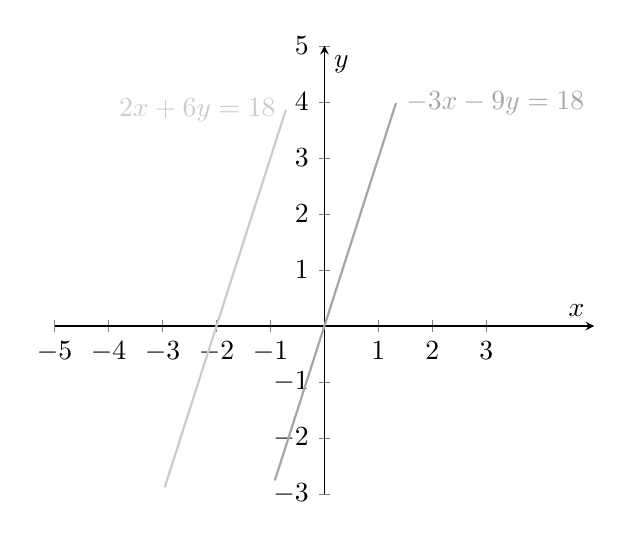
\begin{tikzpicture}
		\begin{axis}[
			xmax=5,
			xmin=-5,
			ymax=5, 
			ymin=-3,
			restrict y to domain=-3:4,
			samples=50,
			xtick={-5,-4,...,3},
		  	ytick={-3,-2,...,5},
		  	xlabel={$x$},
		  	ylabel={$y$}, 
			axis y line=center,
			axis x line=center,
		]
		  \addplot[gray!70,thick] (x,3*x) node [right] {\(-3x - 9y = 18\)};
		  \addplot[gray!40, thick] (x,3*x + 6) node [left] {\(2x + 6y = 18\)};
		\end{axis}
		\end{tikzpicture}
		\end{center}
		\caption{Grafico de las relaciones \(-3x-9y=18\) y \(2x+6y=0\).+} 
		\end{figure}

		Supongamos ahora que existe una solución al sistema de
		ecuaciones y despejemos \(x\) en función a \(y\) obtenemos para obtener
		que
		\[
			2x + 6y = 0 \iff x = -3y,
		\]
		Sustituyendo en la segunda ecuación obtenemos que:
		\[
			-3(-3y) - 9y = 18 \iff 9y - 9y = 18 \iff 0 = 18.
		\]
		Que evidentemente es una contradicción, que provino de asumir que
		nuestro sistema de ecuaciones tenia solución. 


\section{Teoría de conjuntos}


	[El conjunto de los números naturales]
	\[ \{0,1,2,3,4,5,6,7,\ldots\} = \mathbb{N} \]
	
	[El conjunto de los números enteros] 
	\[ {\{\ldots,-4,-3,-2,-1,0,1,2,3,4,\ldots\} = \mathbb{Z}} \]
	
	[El conjunto de los números racionales] 
	\[
		\left\{\ldots,-\frac{2}{2},-\frac{1}{2},0,\frac{1}{2}\ldots \right\} = \mathbb{Q}
	\]

	[El conjunto de los números reales] 
	\[
		\{\ldots-\frac{1}{2},0,(0.99999\ldots),3,\pi,\phi,\ldots\} = \mathbb{R}
	\]

	[Definición por extensión de un conjunto] 
	\[
		\{\text{a}, 2, 0\},\ \{\pi, 2, -2\},\ \{0, 0, 0\}
	\]


	[Definición por compresión del conjunto de los números pares]
	\begin{align}
		A 
		&= \{n\ \text{en los naturales}\  \text{tal que}\ n=2x\ \text{para toda}\ x\ \text{en } \mathbb{N} \}\\
		&= \{n \in \textbf{N}  \mid n=2x\ \text{para toda}\ x\in \mathbb{N} \}\\
		&= \{0,2,4,6,8,\ldots\} \\
		&= \text{Los números pares.}
	\end{align}

	[Definición por compresión de los números impares]
	\begin{align}
		A 
		&= \{n\ \text{en los naturales}\  \text{tal que}\ n=2x + 1\ \text{para toda}\ x\ \text{en } \mathbb{N} \}\\
		&= \{n \in \textbf{N}  \mid n=2x + 1\ \text{para toda}\ x\in \mathbb{N} \}\\
		&= \{1,3,5,7,9,\ldots\} \\
		&= \text{Los números impares.}
	\end{align}

	[Conjunto universo] Sea \(A = \{x \in \mathbb{N} \mid x=2n,\ \text{para todo}\ n\in\mathbb{N}\}\) 
	entonces el conjunto universo de \(A\) es \(\mathbb{N}\)

	[Conjunto complemento] 

	[Definición por compresión de un conjunto arbitrario]
	\begin{align}
		A 
		&= \{x\ \text{en los reales}\  \text{tal que}\ x=2y + 1\ \text{para toda}\ y\ \text{en } \mathbb{R} \}\\
		&= \{x \in \textbf{R}  \mid x=2y + 1\ \text{para toda}\ x\in \mathbb{R} \}\\
		&= \mathbb{R}
	\end{align}

	[El conjunto vació]:
	\begin{align}
		A 
		&= \{x\ \text{en los reales}\  \text{tal que}\ x=1\ \text{y}\ x=2 \}\\
		&= \{x \in \textbf{R}  \mid x=1\ \text{y}\ x=2 \}\\
		&= \emptyset
	\end{align}


\subsection{Operaciones con conjuntos, unión, intersección, diferencia \\ y suma}


	[Unión de dos conjuntos] Sean \(A = \{1,2,3\}\) y \(B=\{1,3,6\}\) entonces
	\begin{align}
		A \cup B &= \{x \mid x \in A \text{ o } x \in B \} \\
			&= \{x \mid x \in \{1,2,3\} \text{ y } x \in \{1,3,6\} \} \\
			&= \{1,2,3,6\} 
	\end{align}


	[Intersección de dos conjuntos] Sean \(A = \{1,2,3\}\) y \(B=\{1,3,6\}\) entonces
	\begin{align}
		A \cap B &= \{x \mid x \in A \text{ y } x \in B \} \\
			&= \{x \mid x \in \{1,2,3\} \text{ y } x \in \{1,3,6\} \} \\
			&= \{ 1, 3 \} 
	\end{align}

	[Diferencia de conjuntos] Sean \(A = \{1,2,3\}\) y \(B=\{1,3,6\}\) entonces
	\begin{align}
		A - B &= \{x \mid x \in A \text{ y } x \notin B \} \\
			&= \{x \mid x \in \{1,2,3\} \text{ y } x \notin \{1,3,6\} \} \\
			&= \{2\} 
	\end{align}


	[Conjunto potencia] Sea \(A = \{1,2,3\}\) entonces
	\begin{align}
		\mathcal{P}(A) &= \{X  \mid X \subset A \} \\
			&= \{\emptyset, \{1\}, \{2\}, \{3\}, \{1,2\}, \{1,3\}, \{2,3\}, \{1,2,3\}\} 
	\end{align}

\subsection{Conjuntos numéricos, naturales, enteros, racionales y reales}

\subsection{Clases de conjuntos: conjuntos de partes, particiones}

\subsection{Producto de conjuntos}

\cleardoublepage
\chapter{Segunda evaluación}

\section{Funciones}

\subsection{Definición, dominio, rango, representación gráfica de funciones}

\subsection{Ejemplos de funciones elementales, suma, diferencia, producto y cociente de funciones}

\subsection{Funciones inyectivas, sobreyectivas y biyectivas}

\subsection{Funciones inversas, composición de funciones}

\subsection{Asintotas funciones crecientes y decrecientes}

\subsection{Funciones elementales}

\section{Función lineal}

\subsection{Definición de función lineal}

\subsection{Cálculo de pendiente de una recta}

\subsection{Gráfico de una función lineal}

\subsection{Puntos de corte funciones lineales, gráfica y analíticamente}

\subsection{Resolución gráfica de sistemas de ecuaciones}

\section{Función polinómica}

\subsection{Definición de función polinómica}

\subsection{Álgebra de las funciones polinómicas}

\subsection{Cálculo de kas raíces de una función polinómica}

\subsection{Teorema del resto, regla de Ruffini}

\subsection{Ceros de un polinomio. Factorización de polinomios}

\subsection{Representación gráfica de una función polinómica}

\subsection{Binomio de Newton}

\subsection{Teoría combinatoria}

{\huge ¿Que temas?}

\chapter{Tercera evaluación}

\section{Elementos de la trigonométria}

\subsection{Teorema de Pitágoras}

\subsection{Funciones trigonométricas y sus funciones inversas}

\subsection{Identidades trigonométricas fundamentales}

\subsection{Seno y coseno de la suma y diferencia de ángulos. Ecuaciones trigonométricas}

\subsection{Gráficas de las funciones trigonométricas y sus inversas}

\section{Función exponencial y logarítmica}

\subsection{Función exponencial}

\subsection{Propiedades}

\subsection{Gráfica de la función exponencial}

\subsection{Función logarítmica}

\subsection{Propiedades}

\subsection{Gráfica de la función logarítmica}